\documentclass[a4paper, 11pt]{article}
\usepackage{covington}
\usepackage{amssymb}
\usepackage{amsmath}
\usepackage[catalan]{babel}
\usepackage{graphicx}
\usepackage{eurosym}
\textheight=23.94cm 
\textwidth=17cm 
\topmargin=-1cm 
\oddsidemargin=-0.5cm 
 
\newcommand{\header}[4]{
	\begin{center}
		\rule{\linewidth}{0.5pt}
		
		{\small{#1}}
      
        \vspace{0.2in}
        
		{\large{#2}}
		
        \vspace{0.2in}
        
		{\small{#3}}
		
		\vspace{0.15in}
		
		{#4}
		
		\vspace{-0.1in}
		\rule{\linewidth}{0.6pt}
	\end{center}
}

\begin{document}
 
\header{\sc Barcelona Graduate School of Economics \hfill Master's Degree in Data Science}{\bf Statistical Modeling and Inference $-$ Problem Set \#1}{\sc Miquel Torrens (NIS: 55550)}{October 7\textsuperscript{th}, 2015}
Solution to proposed exercises.\\
% EXERCISE 1
\newline \textbf{\underline{Exercise 1}}\\
\newline A matrix $\mathbf{A}$ is positive semidefinite iff $\mathbf{x}^T \mathbf{A} \mathbf{x} \geq 0$, $\forall \mathbf{x}$. Using this definition and setting $\mathbf{A} = \mathbf{X}^T \mathbf{X}$, we derive:
\begin{eqnarray}
\mathbf{x}^T \mathbf{A} \mathbf{x} = \mathbf{x}^T \left( \mathbf{X}^T \mathbf{X} \right) \mathbf{x} &=& \left( \mathbf{x}^T \mathbf{X}^T \right)  \left( \mathbf{X} \mathbf{x}  \right) \nonumber \\
&=& \left( \mathbf{X} \mathbf{x} \right)^T  \left( \mathbf{X} \mathbf{x}  \right) \nonumber \\
&=& \mathbf{b}^T \mathbf{b} \nonumber \\
&=& ||\mathbf{b}||^2 \nonumber \\
&\geq & 0. \nonumber
\end{eqnarray}
Thus, $ \mathbf{X}^T \mathbf{X}$ is positive semidefinite under such conditions.\\
% EXERCISE 2
\newline \textbf{\underline{Exercise 2}}\\
\newline We can anticipate that one of them will not be significant, i.e. that its sign will be unsignificantly positive or negative, possibly opposite to the sign of the other covariate.\\
\newline The high correlation between \texttt{lcp} and \texttt{lcavol} draws us think that there is high colinearity between them. Thus, when we run the regression one of them will absorbe the largest part of the variance, leaving the highly-correlated covariate statistically insignificant.\\
% EXERCISE 3
\newline \textbf{\underline{Exercise 3}}\\
\newline \textbf{(a) Show that $\mathbf{H} = \mathbf{H}^T$}\\
\newline We have:
\begin{eqnarray}
\mathbf{H} = \mathbf{\Phi} \left( \mathbf{\Phi}^T \mathbf{\Phi} \right)^{-1} \mathbf{\Phi}^T \nonumber
\end{eqnarray}
Its transpose is:
\begin{eqnarray}
\mathbf{H}^T &=& \left( \mathbf{\Phi} \left( \mathbf{\Phi}^T \mathbf{\Phi} \right)^{-1} \mathbf{\Phi}^T \right)^T \nonumber \\
&=& \left( \mathbf{\Phi} \mathbf{\Phi}^{-1} \left( \mathbf{\Phi}^T\right)^{-1}  \mathbf{\Phi}^T \right)^T \nonumber \\
&=& \left( \mathbf{\Phi}^T \right)^T \left( \left( \mathbf{\Phi}^{-1} \right)^T \right)^T \left( \mathbf{\Phi}^{-1} \right)^T \mathbf{\Phi}^T \nonumber \\
&=&\mathbf{\Phi} \mathbf{\Phi}^{-1} \left( \mathbf{\Phi}^T \right)^{-1} \mathbf{\Phi}^T \nonumber \\
&=& \mathbf{\Phi} \left( \mathbf{\Phi}^T \mathbf{\Phi} \right)^{-1} \mathbf{\Phi}^T \nonumber \\
&=& \mathbf{H}. \nonumber
\end{eqnarray}
\textbf{(b) Show that $\mathbf{H} = \mathbf{H}^2$}\\
\newline Given the above definition of $\mathbf{H}$:
\begin{eqnarray}
\mathbf{H}^2 = \mathbf{H} \mathbf{H} &=& \left( \mathbf{\Phi} \left( \mathbf{\Phi}^T \mathbf{\Phi} \right)^{-1} \mathbf{\Phi}^T \right) \left( \mathbf{\Phi} \left( \mathbf{\Phi}^T \mathbf{\Phi} \right)^{-1} \mathbf{\Phi}^T \right) \nonumber \\
&=& \mathbf{\Phi} \left[ \left( \mathbf{\Phi}^T \mathbf{\Phi} \right)^{-1} \left( \mathbf{\Phi}^T \mathbf{\Phi} \right) \right] \left( \mathbf{\Phi}^T \mathbf{\Phi} \right)^{-1} \mathbf{\Phi}^T \nonumber \\
&=& \mathbf{\Phi} \mathbf{I} \left( \mathbf{\Phi}^T \mathbf{\Phi} \right)^{-1} \mathbf{\Phi}^T \nonumber \\
&=& \mathbf{\Phi} \left( \mathbf{\Phi}^T \mathbf{\Phi} \right)^{-1} \mathbf{\Phi}^T \nonumber \\
&=& \mathbf{H}.  \nonumber
\end{eqnarray}
\textbf{(c) Show that} $\text{tr}(\mathbf{H}) = M+1$ \textbf{.}\\
\newline We use the properties of the trace to solve this:
\begin{eqnarray}
\text{tr}(\mathbf{H}) &=& \text{tr} \left( \mathbf{\Phi} \left( \mathbf{\Phi}^T \mathbf{\Phi} \right)^{-1} \mathbf{\Phi}^T \right) \nonumber \\
&=& \text{tr} \left( \mathbf{\Phi}^T \mathbf{\Phi} \left( \mathbf{\Phi}^T \mathbf{\Phi} \right)^{-1} \right) \nonumber \\
&=& \text{tr} \left(\mathbf{I}_{M+1} \right) \nonumber \\
&=& M+1. \nonumber
\end{eqnarray}
% EXERCISE 4
\newpage
\textbf{\underline{Exercise 4}}\\
\newline Plot 1:\\
\begin{center}
\end{center}
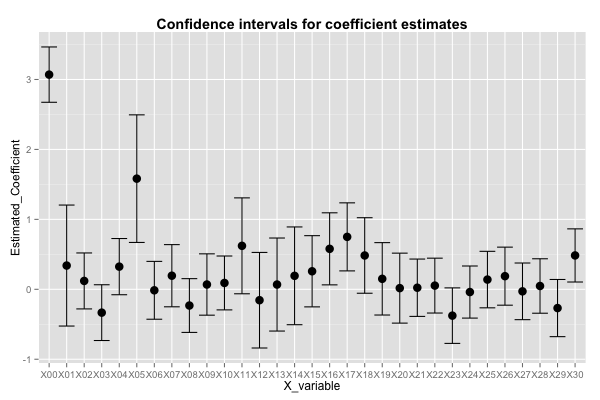
\includegraphics[scale=0.7]{ps1_plot1.png}
\newline Plot 2:\\
\begin{center}
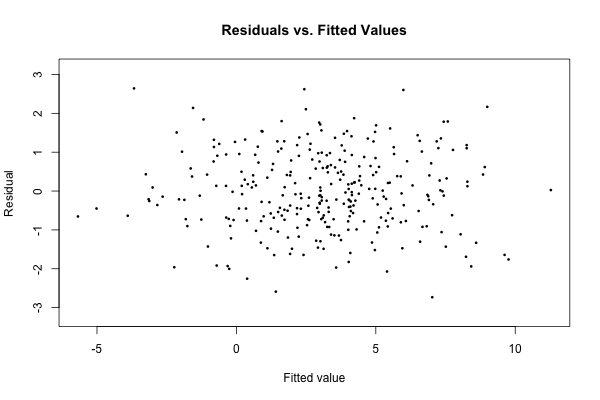
\includegraphics[scale=0.7]{ps1_plot2.png}
\end{center}
Plot 3:\\
\begin{center}
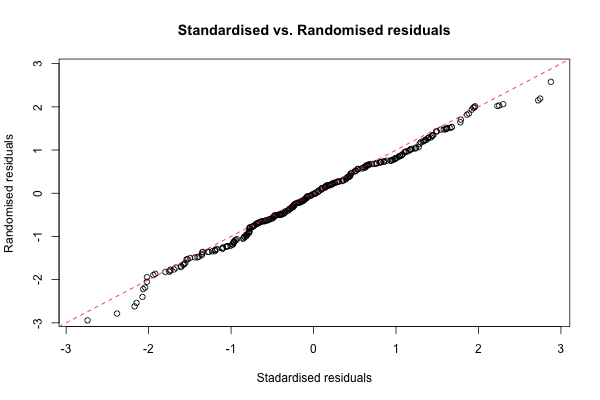
\includegraphics[scale=0.7]{ps1_plot3.png}
\end{center}
% PROBLEM SET 1 (PART 2)
% EXERCISE 5
\newpage
\textbf{\underline{Exercise 5}}\\
\newline As stated in the slides, note that $\mathbf{V}_{r} \mathbf{V}_{r}^{T}$ is the hat matrix in the general case:\\
\begin{eqnarray}
\mathbf{\Phi} \mathbf{w}^{*} = \mathbf{V}_{r} \theta_{MLE} = \mathbf{V}_{r} \mathbf{V}_{r}^{T}  \mathbf{t} = \mathbf{H} \mathbf{t} \nonumber
\end{eqnarray}
So we need to prove that $\mathbf{H}$ is a projection matrix. In mathematical terms, it means it must satisfy the following prperty:
\begin{eqnarray}
\mathbf{H} = \mathbf{H}^2 \nonumber
\end{eqnarray}
Afterwards, we shall prove that $\text{tr}\left( \mathbf{V}_r \mathbf{V}_{r}^{T} \right) = r$.\\
\newline First of all let's prove it is a projection matrix:
\begin{eqnarray}
\mathbf{H}^2 = \mathbf{H} \mathbf{H} = \left( \mathbf{V}_r \mathbf{V}_{r}^{T} \right) \left( \mathbf{V}_r \mathbf{V}_{r}^{T} \right) = \mathbf{V}_r \left( \mathbf{V}_{r}^{T} \mathbf{V}_r \right) \mathbf{V}_{r}^{T}  =  \mathbf{V}_r \mathbf{I}_r \mathbf{V}_{r}^{T} = \mathbf{V}_r \mathbf{V}_{r}^{T} = \mathbf{H} \nonumber
\end{eqnarray}
Thus, this is a projection matrix. Note that we can use $\mathbf{V}_{r}^{T} \mathbf{V}_r = \mathbf{I}_r$ because we know that as part of the singular value decomposition $\mathbf{V}_r$ is by definition an orthogonal matrix, and so that its columns are orthogonal to each other. They are actually orthonormal, meaning that they are unit vectors.\\
\newline This is useful when calculating the trace. Since $\mathbf{V}_r$ is orthogonal and made up of unit vectors, all elements in the diagonal of the product $\mathbf{V}_{r}^{T} \mathbf{V}_r$ are equal to one and thus $\text{tr}\left( \mathbf{V}_r \mathbf{V}_{r}^{T} \right) = \sum_{i=1}^r v_{ii} =  \sum_{i=1}^r 1 = r$, where $v_{ii}$ denotes the diagonal value of the resulting matrix $\mathbf{V}_{r}^{T} \mathbf{V}_r$.\\
% EXERCISE 6
\newpage
\textbf{\underline{Exercise 6}}\\
\newline We shall derive the normal equation for a regression model written as:
\begin{eqnarray}
\mathcal{N} \left( \mathbf{t} | \mathbf{\Phi} \mathbf{w}, (q \mathbf{D})^{-1} \right) = \frac{1}{(2 \pi)^{\frac{D}{2}}} (q \mathbf{D})^{-\frac{1}{2}} \exp \left( -\frac{1}{2} (\mathbf{t} - \mathbf{\Phi} \mathbf{w} )^{T} q \mathbf{D} (\mathbf{t} - \mathbf{\Phi} \mathbf{w} ) \right) \nonumber
\end{eqnarray}
For the sake of simple notation we denote this function simply as $\mathcal{N}$. We compute its log-likelihood function:
\begin{eqnarray}
\prod_N \mathcal{N} &=& \frac{1}{(2 \pi)^{\frac{ND}{2}}} (q \mathbf{D})^{-\frac{N}{2}} \exp \left( -\frac{1}{2} q \sum_N (\mathbf{t} - \mathbf{\Phi} \mathbf{w} )^{T} \mathbf{D} (\mathbf{t} - \mathbf{\Phi} \mathbf{w} ) \right) \nonumber \\
\log \prod_N \mathcal{N} &=& C + \frac{N}{2} \log q \mathbf{D} -\frac{1}{2} q (\mathbf{t} - \mathbf{\Phi} \mathbf{w} )^{T} \mathbf{D} (\mathbf{t} - \mathbf{\Phi} \mathbf{w} ) \nonumber \\
-2 \log \prod_N \mathcal{N} &=& C - N \log q \mathbf{D} + q (\mathbf{t} - \mathbf{\Phi} \mathbf{w} )^{T} \mathbf{D} (\mathbf{t} - \mathbf{\Phi} \mathbf{w} ) \nonumber 
\end{eqnarray}
Where $C$ denotes all constant terms that will disappear during the maximization step. To find the normal equation we will only need to maximize with respect to $\mathbf{w}$. The problem therefore is the following:
\begin{eqnarray}
\max_{\mathbf{w}} -2 \log \prod_N \mathcal{N}  \nonumber
\end{eqnarray}
Before differentiating, we shall develop a little bit the terms involving $\mathbf{w}$:
\begin{eqnarray}
(\mathbf{t} - \mathbf{\Phi} \mathbf{w} )^{T} \mathbf{D} (\mathbf{t} - \mathbf{\Phi} \mathbf{w} ) &=& \mathbf{t}^T \mathbf{D} \mathbf{t} - \left( \mathbf{\Phi} \mathbf{w} \right)^{T} \mathbf{D} \mathbf{t} - \mathbf{t}^T \mathbf{D} \left( \mathbf{\Phi} \mathbf{w} \right) - \left( \mathbf{\Phi} \mathbf{w} \right)^T \mathbf{D} \left( \mathbf{\Phi} \mathbf{w} \right) \nonumber \\
&=& \mathbf{t}^T \mathbf{D} \mathbf{t} - 2 \mathbf{t}^T \mathbf{D} \mathbf{\Phi} \mathbf{w} - \mathbf{w}^T \mathbf{\Phi}^T \mathbf{D} \mathbf{\Phi} \mathbf{w} \nonumber
\end{eqnarray}
To maximize the objective function note that we can just differentiate this term, as the rest will cross out once set to zero:
\begin{eqnarray}
\frac{\partial (-2 \log \prod_N \mathcal{N})}{\partial \mathbf{w}} = 0 \Leftrightarrow \frac{\partial \left( \mathbf{t}^T \mathbf{D} \mathbf{t} - 2 \mathbf{t}^T \mathbf{D} \mathbf{\Phi} \mathbf{w} - \mathbf{w}^T \mathbf{\Phi}^T \mathbf{D} \mathbf{\Phi} \mathbf{w} \right)}{\partial \mathbf{w}} = 0 \nonumber
\end{eqnarray}
Differentiating:
\begin{eqnarray}
-2 \mathbf{t}^T \mathbf{D} \mathbf{\Phi} + \mathbf{w}^T \left( \mathbf{\Phi}^T \mathbf{D} \mathbf{\Phi} + \left( \mathbf{\Phi}^T \mathbf{D} \mathbf{\Phi} \right)^T \right) &=& 0 \nonumber \\
2 \mathbf{t}^T \mathbf{D} \mathbf{\Phi} &=& \mathbf{w}^T \left( \mathbf{\Phi}^T \mathbf{D} \mathbf{\Phi} + \left( \mathbf{\Phi}^T \mathbf{D} \mathbf{\Phi} \right)^T \right) \nonumber \\
\mathbf{t}^T \mathbf{D} \mathbf{\Phi} &=& \mathbf{w}^T \mathbf{\Phi}^T \mathbf{D} \mathbf{\Phi} \nonumber \\
\mathbf{w}^T &=& \mathbf{t}^T \mathbf{D} \mathbf{\Phi} \left( \mathbf{\Phi}^T \mathbf{D} \mathbf{\Phi} \right)^{-1} \nonumber \\
\mathbf{w} &=& \left( \mathbf{t}^T \mathbf{D} \mathbf{\Phi} \left( \mathbf{\Phi}^T \mathbf{D} \mathbf{\Phi} \right)^{-1} \right)^T \nonumber \\
\mathbf{w} &=& \left( \mathbf{\Phi}^T \mathbf{D} \mathbf{\Phi} \right)^{-1} \mathbf{\Phi}^T \mathbf{D}^T \mathbf{t} \nonumber
\end{eqnarray}
From this we can obtain the normal equation:
\begin{eqnarray}
\mathbf{\Phi}^T \mathbf{D} \mathbf{\Phi} \mathbf{w} = \mathbf{\Phi}^T \mathbf{D}^T \mathbf{t} \nonumber
\end{eqnarray}
Given that in practice $\mathbf{D}$ is a diagonal matrix, $\mathbf{D} = \mathbf{D}^T$ and so:
\begin{eqnarray}
\mathbf{\Phi}^T \mathbf{D} \mathbf{\Phi} \mathbf{w} = \mathbf{\Phi}^T \mathbf{D} \mathbf{t} \nonumber
\end{eqnarray}
Hence proved.\\
% EXERCISE 7
\newpage
\textbf{\underline{Exercise 7}}\\
\newline We plot the non-zero singular values:\\
\begin{center}
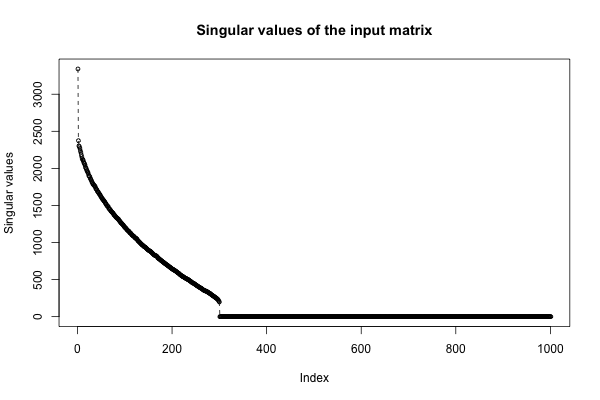
\includegraphics[scale=0.7]{ps1_plot4.png}
\end{center}
Note that some of these values are barely larger than zero, so they are plotted above but visually lie upon the horizontal axis. If we suppress them, the plot looks like this:
\begin{center}
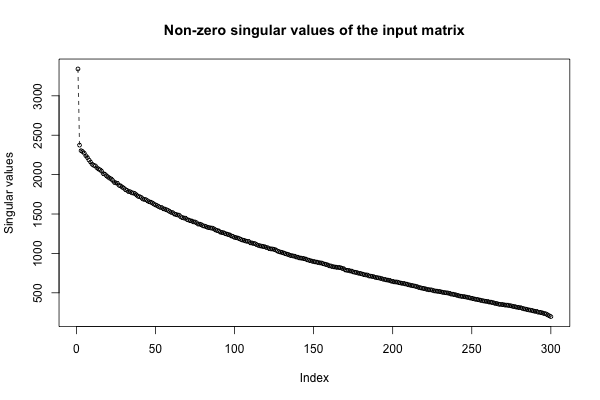
\includegraphics[scale=0.7]{ps1_plot5.png}
\end{center}
The rank of $r$ of the input matrix is precisely the number of singular values greater than zero, which is 300, as you can see above.
\begin{eqnarray}
r = 300. \nonumber
\end{eqnarray}
Now let's perform the principal components regression. We can fit the values using this model to obtain the following results:
\begin{center}
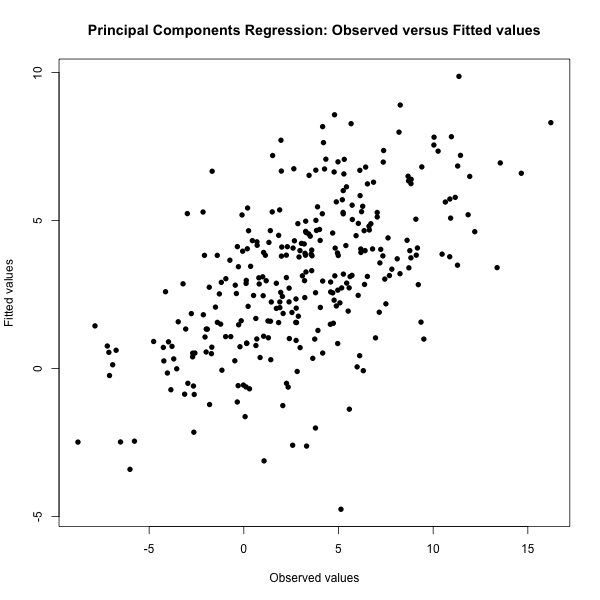
\includegraphics[scale=0.5]{ps1_plot6.png}
\end{center}
We can compare these results with the ones obtained from the model performed in Exercise 3, related to the MLE regression (left picture):
\begin{center}
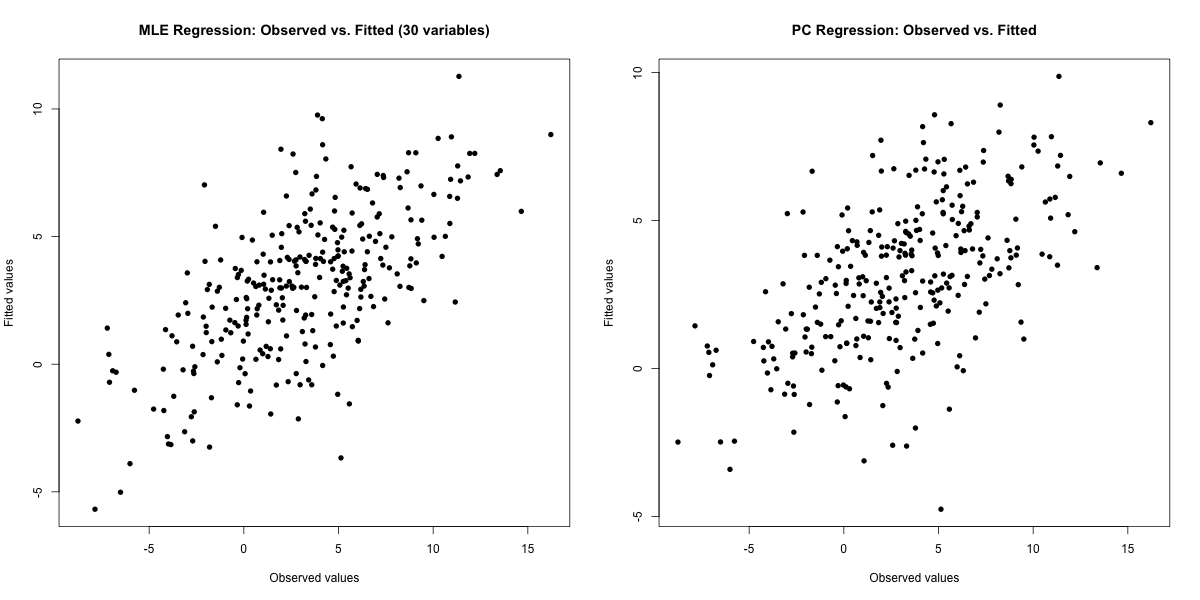
\includegraphics[scale=0.4]{ps1_plot7.png}
\end{center}
It seems that the results for the Principal Components Regression (PCR) are not as compelling as with the MLE Regression. Visually we can already observe some more dispersion of observed versus fitted, and the PCR $R^2$ is lower than the one using the MLE, with $R_{MLE}^2 \approx 0.4275 > 0.3327 \approx R_{PC}^2$. Also, the correlation between observed versus fitted is consequently lower with PCR.








\end{document}